\begin{tikzpicture}[
    node distance=2.5cm,
    featurebox/.style={
        draw,
        inner sep=5pt,
    },
    boxthread/.style={
        inner sep=0pt,
        align=center,
    },
    method/.style={
        draw=black,
        fill=orange!60,
        rounded corners=3pt,
        inner sep=10pt,
        font=\bfseries,
        minimum width=2.3cm,
        align=center
    },
    scale=0.72, transform shape
]

\coordinate (labely) at (0,2cm);

\node[boxthread] (code) {
\begin{minipage}{24mm}
\begin{lstlisting}[style=macrocode,title=A,language=C,captionpos=t]
void main() {
  // ...
}
\end{lstlisting}
\end{minipage}
};
% \node at ($(code.north |- labely)$) {\small (a)};

\node[right=1cm of code] (ast) {
\begin{tikzpicture}[
    level distance=8mm,
    sibling distance=18mm
]
\node {FuncDef}
    child {node {Type}}
    child {
        node {Declarator}
        child {node {Params}}
    }
    child {node {Body}};
\end{tikzpicture}
};
% \node at ($(ast.north |- labely)$) {\small (b)};

\coordinate (feature_pos) at ($(ast.east) + (1cm,0)$);

\def\deltadim{0.05}
\foreach \i in {1,...,3} {
    \pgfmathsetmacro{\displacement}{\i * \deltadim}
    \node[
        featurebox,
        fill=white,
        rounded corners=2.0pt,
        anchor=west
    ] (feature\i) at ($(feature_pos) + (-\displacement,\displacement)$) {
    
\begin{tikzpicture}
        \foreach \i in {0,...,7}
            \fill[blue!60] (0,-0.25*\i) circle (2pt);
    \end{tikzpicture}};
}
% \node at ($(feature1.north |- labely)$) {\small (c)};

\node[
    method,
    right=1.5cm of feature1
] (method) {Method};
% \node at ($(method.north |- labely)$) {\small (d)};

\node (graph) at ($(method.east) + (2.5cm,0)$) {
    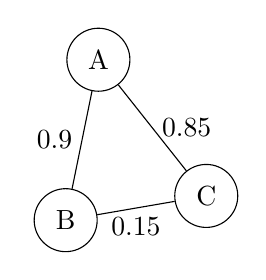
\begin{tikzpicture}[
    node/.style={circle,draw,minimum size=8mm,inner sep=0}
    ]

    \node[node] (A) at (120:1.8cm) {A};
    \node[node] (B) at (200:1.4cm) {B};
    \node[node] (C) at (340:0.5cm) {C};

    \draw (A) -- node[midway,left] {0.9} (B);
    \draw (A) -- node[midway,right] {0.85} (C);
    \draw (C) -- node[midway,below] {0.15} (B);

    \end{tikzpicture}
};
% \node at ($(graph.north |- labely)$) {\small (e)};

\node[
    text=green!60!black,
    right=1cm of graph
] (output) {Output};

\draw[->] ($(code.east)+(0.5,0)$) -- ($(code.east)+(1.0,0)$);
\draw[->] ($(ast.east)+(0.15,0)$) -- ($(ast.east)+(0.65,0)$);
\draw[->] ($(feature1.east)+(0.5,0)$) -- ($(feature1.east)+(1.0,0)$);
\draw[->] ($(method.east)+(0.5,0)$) -- ($(method.east)+(1.0,0)$);
\draw[->] ($(graph.east)+(0.15,0)$) -- ($(graph.east)+(0.65,0)$);

\end{tikzpicture}
